\begin{chapter}{Conclusion and Outlook}
\label{ch:conclusion}

\section{Summary}
In this thesis a very versatile, multi-threaded C++ template library for manifold-valued data was introduced, which extends the original Matlab prototype in a variety of directions. This includes shared memory and SIMD parallelization for IRLS and 
proximal point algorithms, 3D images, 
the Grassmann manifold as well as supporting methods for numerical matrix function derivative computations and OpenGL visualization methods. \\

For the theoretical background some semi-analytic expressions for the derivatives of the squared
distance functions using Kronecker products are provided, which allows a compact and readable implementation.
Furthermore, a short overview about the relevant Grassmann manifold theory was given.\\

The third chapter is a high level documentation of the library and its structure and underlying concepts. It
gives more insights on the software engineering and high performance computing point of view on this thesis 
and also contains some basic tutorials on how to use or even extend the library.\\

Finally, the library's capabilities were demonstrated on many different applications like standard grayscale and color images,
medical DT-MRI data, synthetic $SPD(3)$ and $SO(3)$ data but also examples based on real applications like image orientation
maps and optical flow computation. Aside from these more colorful demonstrations also a performance analysis of the 
library was done to investigate performance bottlenecks of the IRLS minimizer. As main result from this analysis the solution 
of the sparse linear system was identified as the most performance relevant component in the process. This suggests
that the sparse solver do not scale (quasi-)linearly. But also the implementation of the Matrix logarithm Fr\'{e}chet derivative 
had some influence and has potential for further optimization.\\

It was consequently found that IRLS performed slower compared to an also parallelized proximal point algorithm, except for the case of the Grassmannian, due its computationally demanding exponential and logarithm maps. Lastly, in the course of finding further optimization opportunities, the sensitivity
of the computed solution with respect to variations of the original data  was investigated. It could be conclude that 
the resulting error in the solution is locally
confined to a neighborhood around the varied pixel in the original and decays exponentially with the distance from the varied pixel.
A possibility for an extension of the library exploiting this locality of the error is discussed in
the last Section \ref{sec:Recursivecomputationonsubdomains}. Next, however, some more general possibilities are suggested.

\section{Extensions and Improvements} % (fold)
\label{sec:Extensions}
\subsection{Performance}
Since the solution of the sparse linear system is the most performance critical component of the algorithm, new 
solution methods should be tested. In particular, iterative methods could perform better if a good preconditioner
can be found. \\

By making use of the special block-band structure of the Hessian, the MTVMTL implementation avoids the temporary block diagonal 
matrix, containing the tangent space basis transformation, that was used in the Matlab prototype. The tangent space
transformations can instead be applied directly to the pixels of the derivative containers.
In a similar manner, it might also be possible to make the algorithm completely matrix-free by 
implementing a matrix-vector multiplication function for the Hessian matrix, that can be used by iterative solver.
This might save a lot of memory as well as computation time and bring the algorithm closer to the linear complexity
regime.

\subsection{Manifolds and Minimizers}
The first thing that can easily be extended is the support for additional manifolds. Possibilities are, for instance, the Stiefel manifold that
was briefly introduced in section \ref{sub:Grassmanian} or an alternative implementation of the $SPD(n)$ manifold using the Log-Euclidean metric
based on \cite{LogEuclidian}.\\

Also new minimizers could be added. It would be straightforward to utilize the gradient evaluation function already implemented in the functional to
add some gradient descent based algorithm and compare again with IRLS-Newton and proximal point. For new functionals a more detailed suggestion
is provided in the next Section.

\subsection{Functionals} % (fold)
\label{sub:Functionals}
So far isotropic and anisotropic first order TV functionals are implemented in the library. Extensions can be made with respect to the TV part or the fidelity
part of the functional. In the first case this would mean to also include a second order TV term $\mu\int_{\omega}|\nabla^2u|\mathop{dx}$ in the functional.
This prevents the formation of numerical artifacts like the so-called staircasing effects, that might occur in first order TV. Of course also higher orders than second
can be added to the functional. As long as also methods for the evaluation of the functionals gradient and Hessian are provided, the IRLS minimizer class will
work without any changes. \\

The second possibility is the addition of new or different fidelity terms. The purpose of the fidelity term during the minimization is to penalize a TV
regularization that moves too far away from the original picture. However, one can also utilize it for a direct calculation of a dense optical flow field, for
example. This was also done in the application shown in \ref{sub:reconstructionDenseOpticalFlow} but it must be noted that the procedure in the example to computation of the dense flow was rather complicated and indirect.\\

For the direct TV approach, as presented in \cite{SceneFlow}, consider a 2D video sequence $I:\Omega\times [0,T]\to\mathbb{R}$.
Let now $u:\Omega\to\mathbb{R}^2$ denote the displacement vector of the of the pixel $x\in\Omega$. The functional is then given by
\begin{equation}
    J(u)=\int_{\Omega}\left\vert\frac{\partial I}{\partial t}+\nabla I\cdot u\right\vert\mathop{dx}+\lambda TV(u),
\end{equation}
where the first term is the new data term, which implements the so-called optical flow constraint that could be interpreted as a continuity equation for pixels.
Finally, as Lef\'{e}vre and Baillet show in \cite{manifoldFlow}, the functional can be generalized also to flows on some classes of manifolds.
% subsection Functionals (end)

% section Extensions (end)

\section{Recursive computation on subdomains} % (fold)
\label{sec:Recursivecomputationonsubdomains}
From the numerical experiment in Section \ref{sec:Sensitivity} it can be concluded that a local neighborhood of the original picture only affects the form of the minimizer of the function
in its immediate neighborhood. The magnitude of the variation in the minimizer due to the variation of a single pixel in the original data seems to decay exponentially with the
distance from that pixel. \\

This could in principle be exploited by dividing the image into subdomains with a specific small overlap, determined by the error boundaries, and solve each of the smaller 
subproblems individually. Depending on the size of the necessary overlap this could also be employed recursively until a minimal subimage size is reached. Then, after all subproblems
are solved the subpictures are recombined just by cropping all overlapping regions to arrive at the global solution.
As a final example, an extended version of the Lena picture is split in the middle with $50px$ overlap, as shown in Figure \ref{fig:splitting1}.

\begin{figure}[h!]
    \centering
    \subfloat[][Noisy full picture]{
	\label{fig:splitting_full}
	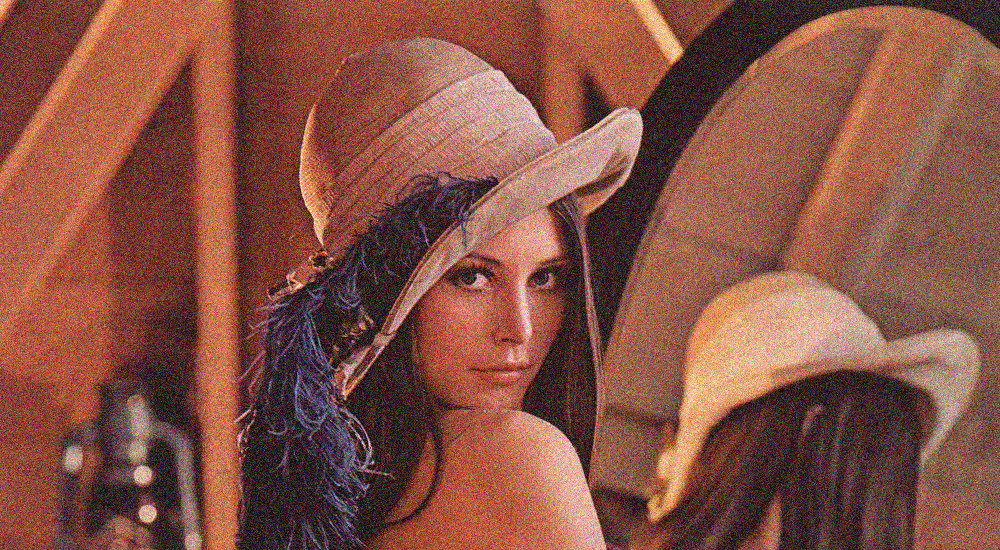
\includegraphics[width=0.475\linewidth]{./figures/experiments/noisy_lena_top.jpg}
    }
    \subfloat[][Noisy left half]{
	\label{fig:splitting_left}
	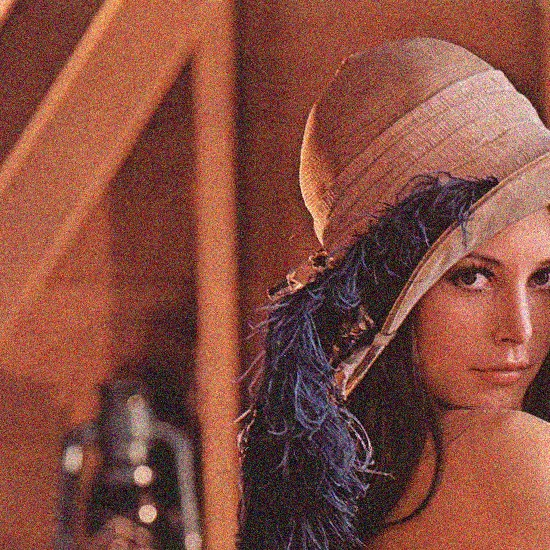
\includegraphics[width=0.25\linewidth]{./figures/experiments/noisy_lena_top1.jpg}
    }
    \subfloat[][Noisy right half]{
	\label{fig:splitting_right}
	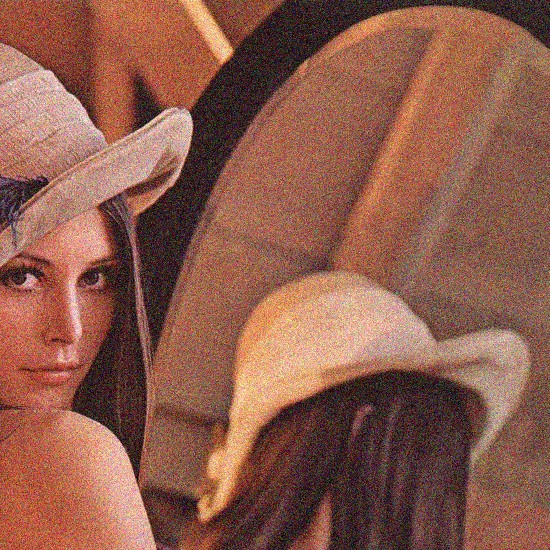
\includegraphics[width=0.25\linewidth]{./figures/experiments/noisy_lena_top2.jpg}
    }\\
    \caption[Splitting the image domain]{Splitting of the Lena picture into two domains
	\subref{fig:splitting_full} Original image "Lena.jpg", $1000\times 550$ px, 8 bit color depth
	\subref{fig:splitting_left} Left half, $550\times 550$
	\subref{fig:splitting_right} Right half $550\times 550$
	\label{fig:splitting1}
    }
\end{figure}
Next, algorithm is applied to the the full picture, which takes 72 seconds, as well as to the two halves, which takes 
33 second for each run. Then the two halves are recombined after cropping away the overlap. The results, shown in
Figure \ref{fig:splitting2}, look promising. Of course, at this point some more detailed numerical error analysis
should be performed but just from visual inspection there are no serious problems, like a visible brightness or color gradient for example, of the splitting procedure evident.\\

\begin{figure}[h!]
    \centering
    \subfloat[][]{
	\label{fig:splitting_denoised}
	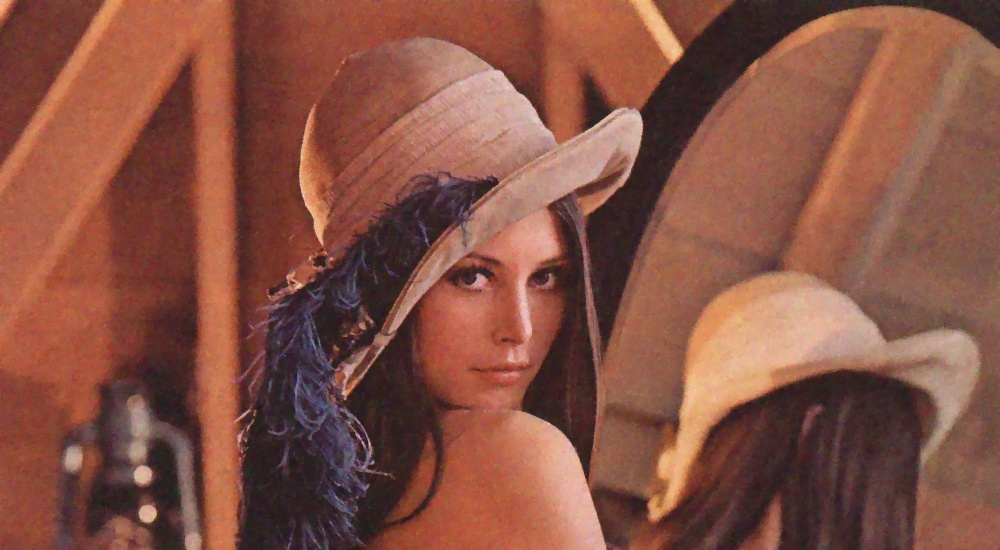
\includegraphics[width=0.5\linewidth]{./figures/experiments/denoised_lena_top.jpg}
    }
    \subfloat[][]{
	\label{fig:splitting_recombined}
	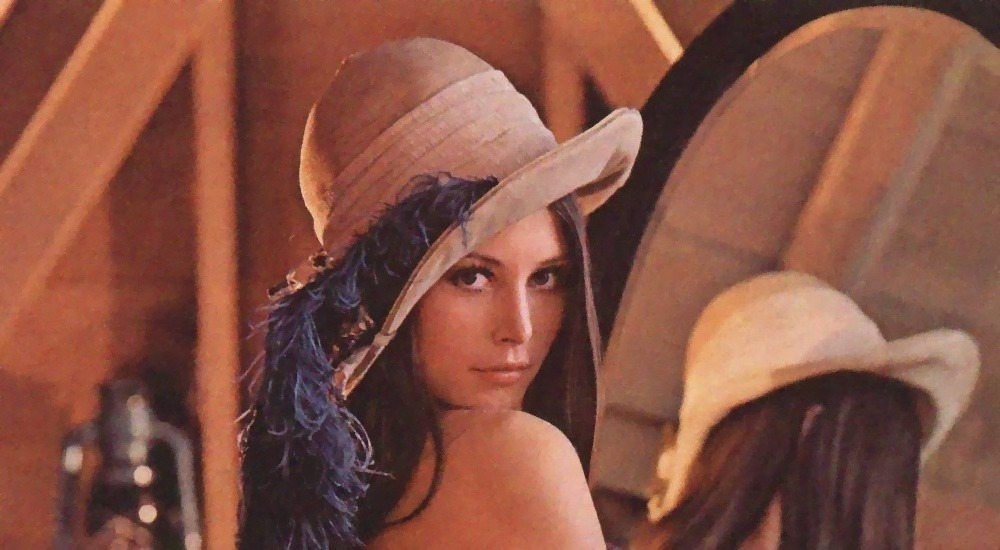
\includegraphics[width=0.5\linewidth]{./figures/experiments/recombined_lena_top.png}
    }\\
    \caption[Comparison full domain versus splitted domain denoising]{Comparison between the denoising
    over the full domain and denoising over two subdomains
	\subref{fig:splitting_denoised} Denoised full picture
	\subref{fig:splitting_recombined} Recombined, denoised picture halves
	\label{fig:splitting2}
    }
\end{figure}

The advantages of this procedure are firstly, that even though there is some overhead from this procedure, a collection of smaller subproblems can be usually solved faster than one big problem and have a lower memory consumption. The speed up in the above example
is not very large (66 versus 72 seconds), which is also to be expected from the subquadratic time complexity measured in 
Section \ref{sub:TimeComplexity}. Nevertheless, the main point is not about the speed up of serial-solving the subproblems but
the lower memory demand allowing yet larger images to be processed.\\

Secondly, this splitting scheme can also be used to introduce an additional layer of parallelism in the from of distributed memory, 
many core parallelization. Each subproblem can be assigned to a different node that in turn locally applies multi-threading.
Building such a distributed computing architecture on top of the solver, a significant speed up can be reached, because except
from splitting and recombination there is no need for communication between the nodes during the TV minimization.
% section Recursive computation on subdomains (end)

\end{chapter}
